%%%%%%%%%%%%%%%%%%%%%%%%%%%%%%%%%%%%%%%%%
% baposter Landscape Poster
% LaTeX Template
% Version 1.0 (11/06/13)
%
% baposter Class Created by:
% Brian Amberg (baposter@brian-amberg.de)
%
% This template has been downloaded from:
% http://www.LaTeXTemplates.com
%
% License:
% CC BY-NC-SA 3.0 (http://creativecommons.org/licenses/by-nc-sa/3.0/)
%
%%%%%%%%%%%%%%%%%%%%%%%%%%%%%%%%%%%%%%%%%

%----------------------------------------------------------------------------------------
%	PACKAGES AND OTHER DOCUMENT CONFIGURATIONS
%----------------------------------------------------------------------------------------


\documentclass[landscape,a0paper,fontscale=0.31]{baposter} % Adjust the font scale/size here
\usepackage[english, serbian c]{babel}
\usepackage[utf8]{inputenc}
\usepackage{float}
\usepackage{floatrow}
\usepackage[T2A]{fontenc}
\usepackage[colorlinks=true, allcolors=blue]{hyperref}
\usepackage{graphicx} % Required for including images
\graphicspath{{figures/}} % Directory in which figures are stored

\usepackage{amsmath} % For typesetting math
\usepackage{amssymb} % Adds new symbols to be used in math mode

\usepackage{breqn}  % Used for breaking equations on multiple lines


\usepackage{booktabs} % Top and bottom rules for tables
\usepackage{enumitem} % Used to reduce itemize/enumerate spacing
\usepackage{palatino} % Use the Palatino font
\usepackage[font=small,labelfont=bf]{caption} % Required for specifying captions to tables and figures

\usepackage{multicol} % Required for multiple columns
\setlength{\columnsep}{1.5em} % Slightly increase the space between columns
\setlength{\columnseprule}{0mm} % No horizontal rule between columns

\usepackage{tikz} % Required for flow chart
\usetikzlibrary{shapes,arrows} % Tikz libraries required for the flow chart in the template

\newcommand{\compresslist}{ % Define a command to reduce spacing within itemize/enumerate environments, this is used right after \begin{itemize} or \begin{enumerate}
\setlength{\itemsep}{1pt}
\setlength{\parskip}{0pt}
\setlength{\parsep}{0pt}
}

\definecolor{lightblue}{rgb}{0.145,0.6666,1} % Defines the color used for content box headers

\begin{document}

\begin{poster}
{
headerborder=closed, % Adds a border around the header of content boxes
colspacing=1em, % Column spacing
bgColorOne=white, % Background color for the gradient on the left side of the poster
bgColorTwo=white, % Background color for the gradient on the right side of the poster
borderColor=lightblue, % Border color
headerColorOne=black, % Background color for the header in the content boxes (left side)
headerColorTwo=lightblue, % Background color for the header in the content boxes (right side)
headerFontColor=white, % Text color for the header text in the content boxes
boxColorOne=white, % Background color of the content boxes
textborder=roundedleft, % Format of the border around content boxes, can be: none, bars, coils, triangles, rectangle, rounded, roundedsmall, roundedright or faded
eyecatcher=true, % Set to false for ignoring the left logo in the title and move the title left
headerheight=0.1\textheight, % Height of the header
headershape=roundedright, % Specify the rounded corner in the content box headers, can be: rectangle, small-rounded, roundedright, roundedleft or rounded
headerfont=\Large\bf\textsc, % Large, bold and sans serif font in the headers of content boxes
%textfont={\setlength{\parindent}{1.5em}}, % Uncomment for paragraph indentation
linewidth=2pt % Width of the border lines around content boxes
}
%----------------------------------------------------------------------------------------
%	TITLE SECTION 
%----------------------------------------------------------------------------------------
%
{\includegraphics[height=9.5em]{matf.png}} % First university/lab logo on the left
{\bf\textsc{О култури, технологији и глобалним градовима}} % Poster title
{\textsc{ Сара Селаковић \\  mi17017@alas.matf.bg.ac.rs \\   Семинарски рад у оквиру курса Рачунарство и друштво}} % Author names and institution
{\includegraphics[height=9.5em]{matf.png}} % Second university/lab logo on the right

\headerbox{Концепт глобалних градова}{name=konceptgg,column=0,span=4,row=0}{
Данас jе могуће имати, на пример,  кухиње и ресторане разних удаљених места у истом граду, тако да нема смисла препуштати град другом за такве услуге или искуства. Трендови ширења искустава у jедном граду негативно утичу на културни и урођени идентитет градова. То на краjу доводи до хомогених пеjзажа што води до погоршања културне вредности града. Када се то догоди, граду jе тада тешко да привуче ново тржиште културног туризма. Овакве стратегиjе постављаjу \textit{концепт глобалних градова}. 
}

\headerbox{Последице технологије у туризму}{name=posledice,column=0,row=1,span=1, below=konceptgg}{
Улога технологиje може имати негативне последице jер може довести до хомогености урбаног ткива кроз популарне модернистичке идеологиjе и методе планирања. Већина архитектонских дела је демонтирана, рушена, деформисана или подвргнута реновирању. Такве праксе угрожаваjу посебност и културне аспекте градова и негативно утичу на њихову атрактивност у погледу културног туризма. 
\\

\begin{center}
\includegraphics[width=1\linewidth]{posta.jpg}
\captionof{figure}{Пошта у Београду пре и после реновирања}
\end{center}

\vspace{1.8em}
\hspace{1.8em}
}

\headerbox{Закључак}{name=zakljucak,column=0,span=4, above=bottom}{ 
Улога технологиjе у градовима мора бити пажљиво интегрисана, jер мешање различитих култура, ико се цени, мора бити пажљиво
урађено. Културни атрибути се не смеjу негирати нити заjедно груписати, jер као такви могу брзо да подстакну стварање хомогених простора.
}

\headerbox{Апликациjе за промовисање садржаjа}{name=aplikacije,column=2,span=1,row=0,below=konceptgg, above=zakljucak}{
Користе за приказивање информациjа попут
културних календара, културних локациjа и дељења слика уживо из различитих делова градова. Развиjене су платформе за резервисање
седишта, продаjу карата, вожњу таксиjем по градовима и многе друге.
\\

\begin{center}
\includegraphics[height=12em]{eventbr.jpg}
\captionof{figure}{Евентбрајт апликација: омогућава организаторима да путем ње поставе информациjе о предстоjећим догађаjима}
\end{center}

\begin{center}
\includegraphics[height=15em]{vamos.png}
\captionof{figure}{Вамос апликација за такси услуге}
\end{center}
}

\headerbox{Брендирање градова}{name=brendiranje,column=3,span=1,row=0,below=konceptgg, above = zakljucak}{
Наjпознатиjи од таквих брендова су: I Love New York, IAMSTERDAM, Nothing normal ever changed a damn thing (Хелсинки), Let’s Make it Happen
(Луксембург), итд. Овакво брендирање се користи као алат за покретање концепта jединственог идентитета са коjим би се могли повезати они коjи бораве или посећуjу град.
\\

\begin{center}
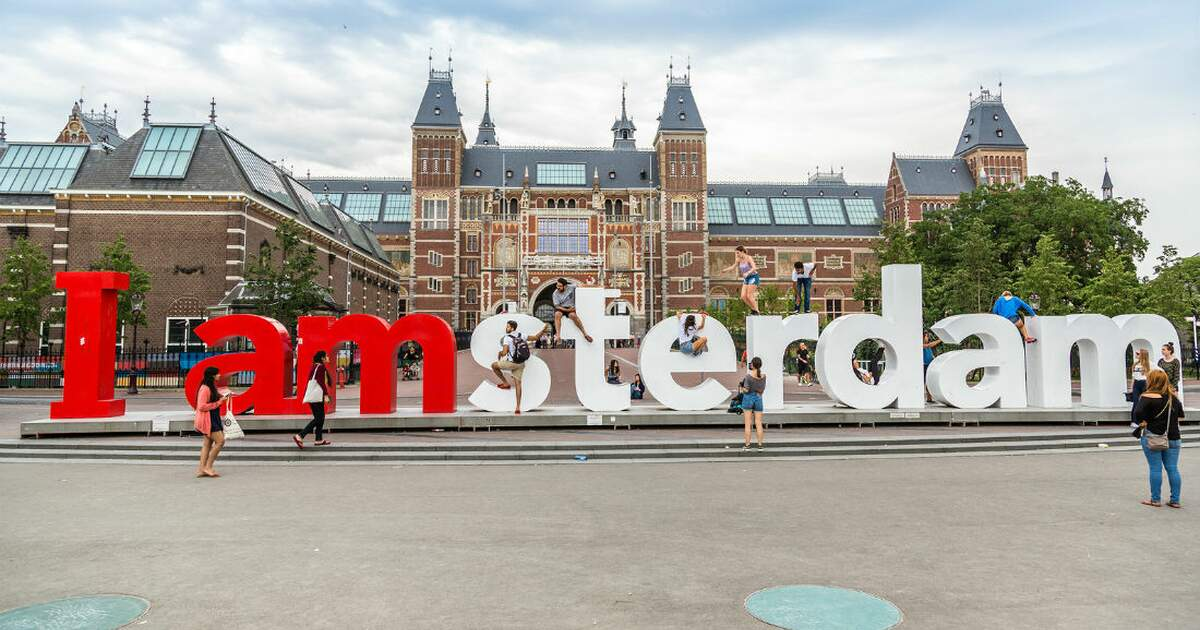
\includegraphics[height=11em]{amsterdam.jpg}
\captionof{figure}{Брендирање Амстердама}
\end{center}

\begin{center}
\includegraphics[height=15.5em]{luxair.jpg}
\captionof{figure}{Брендирање Луксембурга}
\end{center}
}

\headerbox{Превазилажење хомогености}{name=prevazilazenjeh,column=1,row=0, below=konceptgg}{ 
Технологија омогућава поновно успостављање изгубљених наслеђа претварајући их у облике који привлаче модерне културне туристе. \textit{Проширена стварност} (augmented reality) и \textit{виртуелна реалност} (virtual reality) су међу најпопуларнијим технологијама које градови користе да би побољшали своју атрактивност. Помоћу њих, може се приказати културно наслеђе у облику текста, видеа и сл. Тиме градови повећаваjу вредност услуга коjе нуде, jер путницима пружају слободу да персонализуjу садржаj по свом укусу како желе.
\\

\begin{center}
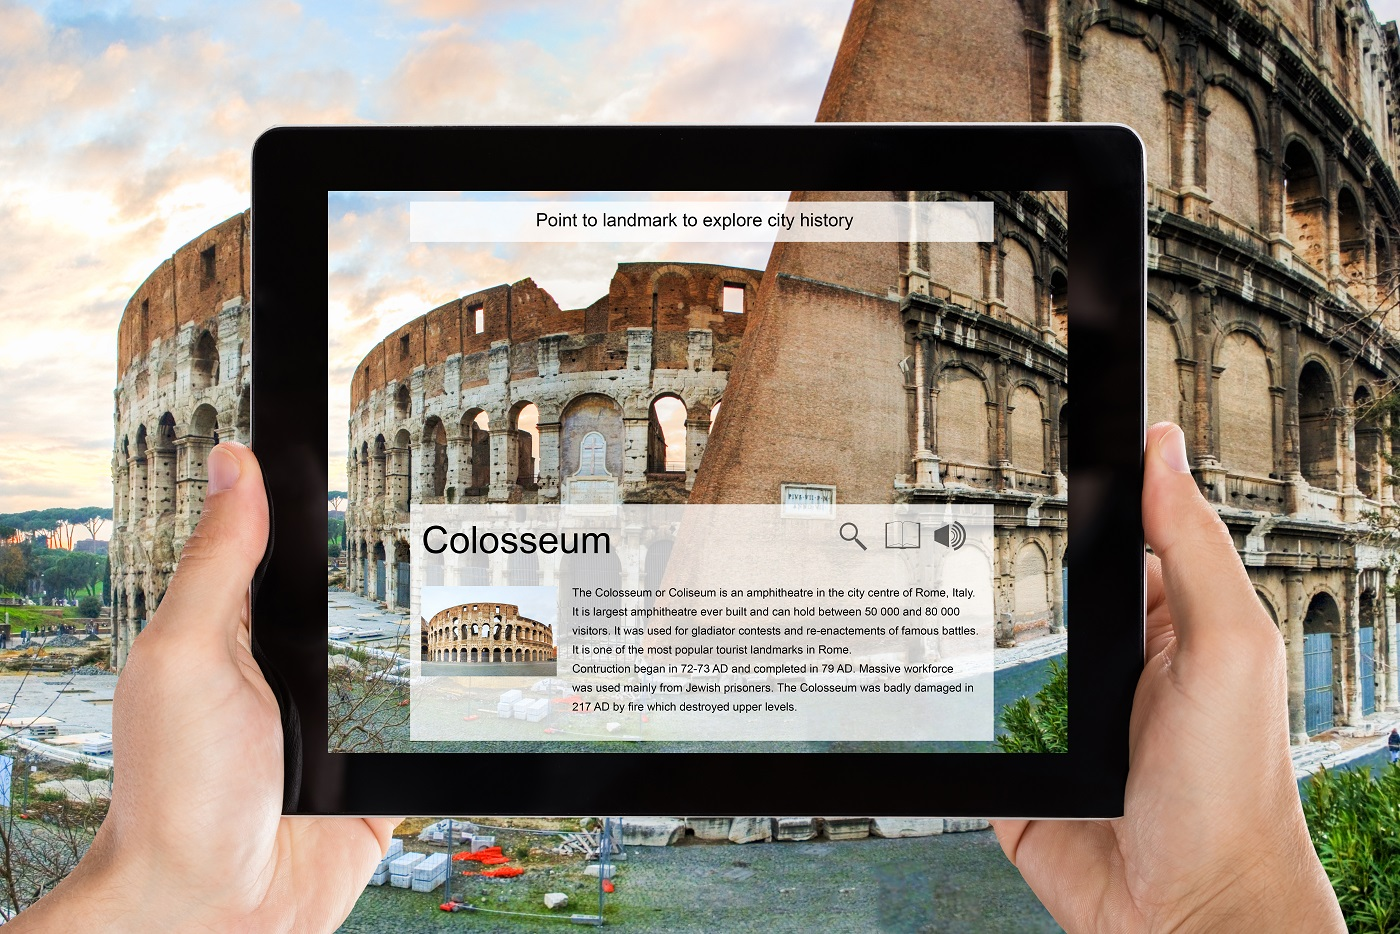
\includegraphics[height=12.6em]{ar.jpg}
\captionof{figure}{АР технологија}
\end{center}

\begin{center}
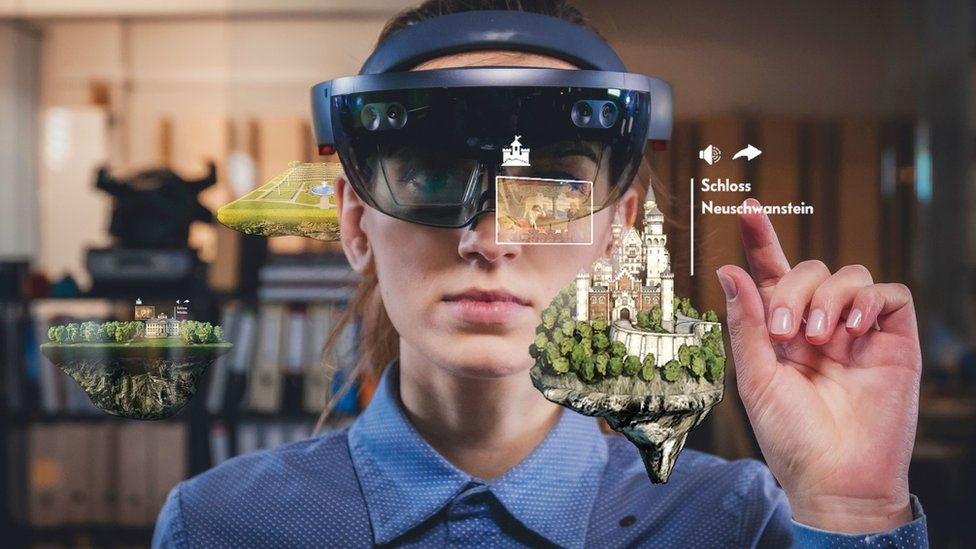
\includegraphics[height=10.6em]{vr.jpg}
\captionof{figure}{ВР технологија}
\end{center}

\vspace{1.8em}
\hspace{1.8em}
}

%----------------------------------------------------------------------------------------

\end{poster}

\end{document}
